\documentclass{article}

\usepackage{color}
\usepackage[utf8]{inputenc}
\usepackage[finnish]{babel}
\usepackage{hyperref}
\usepackage{amsmath}
\usepackage{listings}
\usepackage{pgfplots}

\lstset{
	identifierstyle=\ttfamily,
    breaklines=true,
    keywordstyle=\color[rgb]{0,0,1},
    commentstyle=\color[rgb]{0.133,0.545,0.133},
    stringstyle=\color[rgb]{0.627,0.126,0.941},
	language=Python
}

\pgfplotsset{width=11cm}

\newcommand{\BigO}[1]{\ensuremath{\operatorname{O}\bigl(#1\bigr)}}

\setlength{\parindent}{0.0in}
\setlength{\parskip}{0.1in}

\begin{document}
\title{Tiralabra 2013 periodi III \\ Testausdokumentti}
\author{Mika Viinamäki}
\maketitle

\section{Testauksen osat}
Ohjelmaan liittyvät testit voidaan jakaa kahteen eri osaan:

\begin{itemize}
\item Yksikkötestit, jotka testaavat että ohjelma toimii oikein.
\item Suorituskykytestit, jotka testaavat ohjelman suorituskykyä erilaisilla syötteillä.
\end{itemize}

\section{Yksikkötestit}
Yksikkötestit testaavat algoritmin toimintaa kokonaisuudessaan sekä siihen liittyvien pienempien palasten toimintaa erikseen. Algoritmin osalta testit eivät testaa että LZW-pakkauksen muoto on sellainen niinkuin pitääkin - testeille riittää, että testidata on identtinen pakkaamisen ja purkamisen jälkeen ja että se vie pakattuna tietyn verran vähemmän tilaa kuin alkuperäinen data.

Yksikkötestit voi ajaa vaikkapa komennolla \texttt{mvn test} Netbeans-projektin juuressa tai avaamalla projekti Netbeansissa ja ajamalla testit sen kautta.

\section{Suorituskykytestit}

Suorituskykytestejä on muutamia erilaisia:
\begin{itemize}
\item \texttt{kauhsa.compression.lzw.benchmarks.PerformanceBenchmark}, joka testaa pakkaus- ja purkunopeutta erilaisilla syötteillä ja asetuksilla
\item \texttt{kauhsa.compression.lzw.benchmarks.CompressionBenchmark}, joka testaa miten tiiviisti tieto pakkautuu erilaisilla syötteillä ja asetuksilla
\item \texttt{kauhsa.utils.hashmap.HashMapBenchmark}, joka testaa hajautustaulun tehokkuutta
\end{itemize}

Nopeutta testaavat suorituskykytestit käyttävät Caliper\footnote{\url{http://code.google.com/p/caliper/}}-nimistä frameworkia, joka on suunniteltu microbenchmarkien tekemiseen. Nopeustestit tehdään ehkä tarpeettomankin suurella tarkkuudella, ja tästä johtuen niiden ajaminen saattaa kestää todella kauan --- jopa puolesta tunnista tuntiin. En kuitenkaan löytänyt frameworkista mitään asetuksia mitkä olisivat ratkaisevasti parantanut testien ajamisnopeutta.

Suorituskykytestit voidaan ajaa vaikkapa ajamalla kyseinen luokka ("Run File") Netbeansin kautta.

\subsection{Pakkaus- ja purkunopeus}
Pakkausnopeustestien tulokset löytyvät kokonaisuudessaan \href{http://microbenchmarks.appspot.com/run/kauhsa@viuhka.fi/kauhsa.compression.lzw.benchmarks.PerformanceBenchmark}{täältä}.

\begin{figure}[h]
\centering
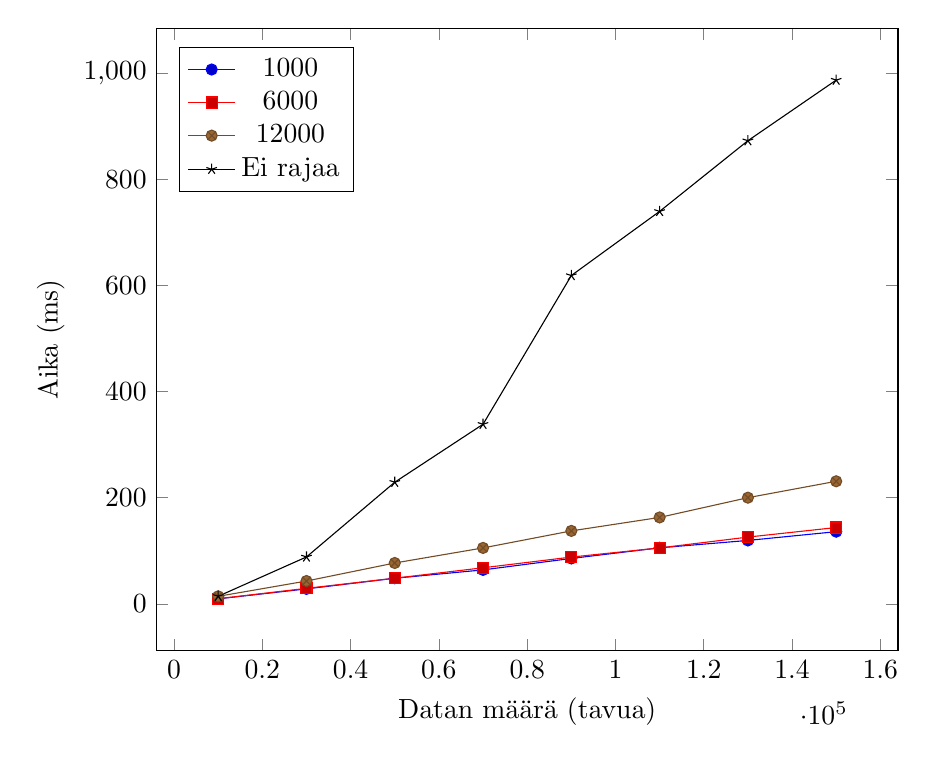
\begin{tikzpicture}
	\begin{axis}[
			xlabel=Datan määrä (tavua),
			ylabel=Aika (ms),
			legend pos=north west]
		
		\addplot coordinates {
			(10000,9.57)
			(30000,28.35)
			(50000,48.37)
			(70000,64.13)
			(90000,85.68)
			(110000,105.72)
			(130000,119.63)
			(150000,136.15)
		};
		\addlegendentry{1000}
		
		\addplot coordinates {
			(10000,9.87)
			(30000,29.34)
			(50000,48.48)
			(70000,68.10)
			(90000,88.29)
			(110000,105.50)
			(130000,125.92)
			(150000,143.95)
		};
		\addlegendentry{6000}

		\addplot coordinates {
			(10000,14.32)
			(30000,43.15)
			(50000,77.13)
			(70000,105.51)
			(90000,137.60)
			(110000,162.98)
			(130000,200.18)
			(150000,231.06)
		};
		\addlegendentry{12000}
		
		\addplot coordinates {
			(10000,14.43)
			(30000,88.49)
			(50000,229.31)
			(70000,338.52)
			(90000,618.74)
			(110000,739.59)
			(130000,872.75)
			(150000,986.94)
		};
		\addlegendentry{Ei rajaa}
		
	\end{axis}
\end{tikzpicture}
\caption{Pakkausnopeus satunnaisesti generoidulla datalla}
\end{figure}

Kuvasta nähdään hyvin, miten sanakirjan rajan poistaminen vaikuttaa pakkausnopeuteen --- testin perusteella se pysyy lineaarisenaniin kauan kun sanakirjalla on jokin raja, mutta rajan poistaminen seurauksena pakkausnopeus hidastuu merkittävästi.

Syynä pakkauksen hidastumiseen nostaessa sanakirjan rajaa lienee hajautustaulun operaatioiden hidastuminen, kun siihen lisättyjen alkioiden määrä kasvaa.

\end{document}